%---------------------------------------------------------------------------

\begin{frame}
	\frametitle{Plan prezentacji}

	\begin{enumerate}
		\item Algorytm Scale Space
		\item Standard OpenCL
		\item Wyniki
	\end{enumerate}

\end{frame}

%---------------------------------------------------------------------------

%Jednym z istotniejszych problemów podczas automatycznego przetwarzania i analizy obrazów jest wybór skali.

%Obrazy mogą być rejestrowane w~różnych skalach.

\begin{frame}
	\frametitle{Algorytm Scale Space}
	\begin{block}{Scale Space}
		Algorytm służący do przedstawiania sygnałów w reprezentacji skali.
	\end{block}
	Można go zastosować do dowolnych sygnałów. Praca skupia się na wykorzystaniu algorytmu do przetwarzania obrazów.

\end{frame}

%---------------------------------------------------------------------------
\begin{frame}
	\frametitle{Podstawy matematyczne}
	
	\begin{center}
		$ g(x,y,\sigma)= \frac{1}{2 \cdot \pi \cdot \sigma ^ {2} }\cdot e^{(-\frac{x^{2} + y^{2}}{2 \cdot \sigma ^{2}})} $

	\begin{figure}[h]
		\begin{center}
			\begin{subfigure}[b]{4.5cm}
				\centering
				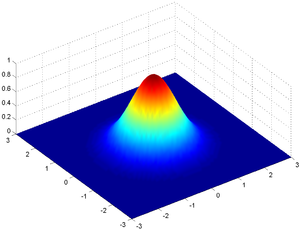
\includegraphics[width=4.5cm]{gaussian2d.png}
			\end{subfigure}
			~
			\begin{subfigure}[b]{4.5cm}
				\centering
				\includegraphics[width=4.5cm]{gaussian2dcoef}
			\end{subfigure}
		\end{center}
	\end{figure}
		
	\end{center}
	
	Do wyznaczenia przestrzeni skali stosuje się filtry Gaussa. 
	
	%Poniżej przedstawiono sposób wyznaczania współczynników filtra w przestrzeni dwuwymiarowej.
	
\end{frame}
%---------------------------------------------------------------------------
\begin{frame}
	\frametitle{Algorytm Scale Space dla obrazów}

	\begin{figure}[h]
		\begin{center}
			\begin{subfigure}[b]{3.5cm}
				\centering
				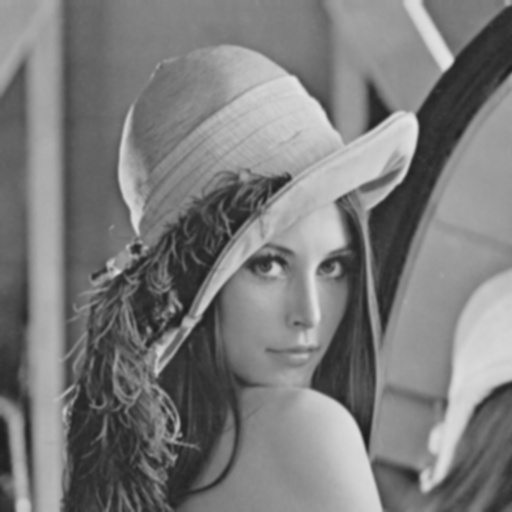
\includegraphics[width=2.5cm]{Lena_scales1.jpg}
				\caption{Obraz oryginalny}
			\end{subfigure}
			~
			\begin{subfigure}[b]{3.5cm}
				\centering
				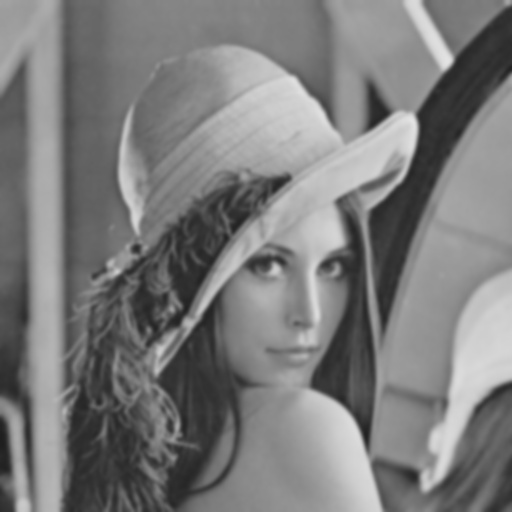
\includegraphics[width=2.5cm]{Lena_scales2.jpg}
				\caption{$\sigma = 0,95$, $N = 3$}
			\end{subfigure}
			~
			\begin{subfigure}[b]{3.5cm}
				\centering
				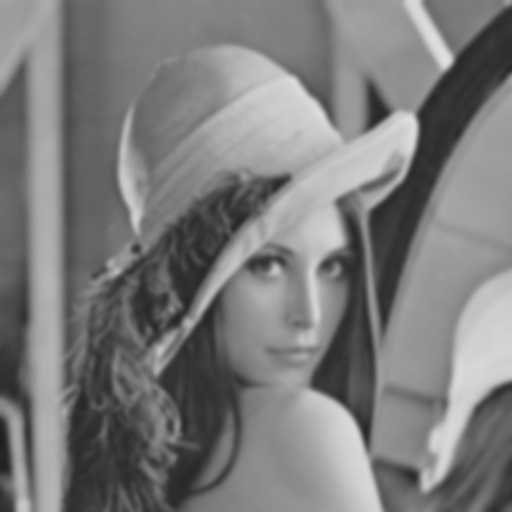
\includegraphics[width=2.5cm]{Lena_scales3.jpg}
				\caption{$\sigma = 1,25$, $N = 5$}
			\end{subfigure}


			\begin{subfigure}[b]{3.5cm}
				\centering
				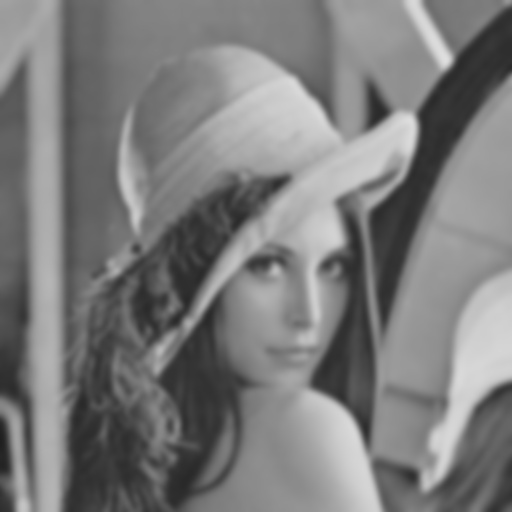
\includegraphics[width=2.5cm]{Lena_scales4.jpg}
				\caption{$\sigma = 1,55$, $N = 7$}
			\end{subfigure}
			~
			\begin{subfigure}[b]{3.5cm}
				\centering
				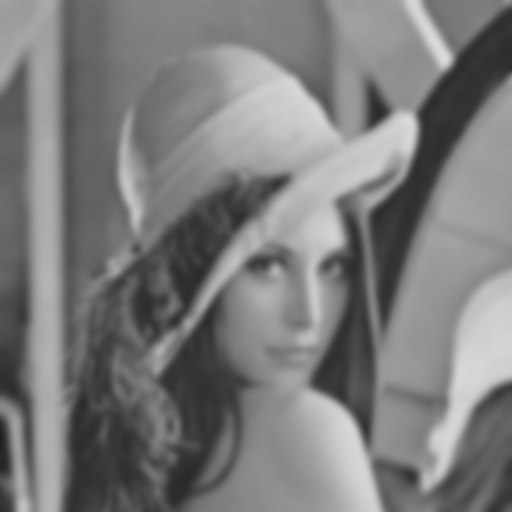
\includegraphics[width=2.5cm]{Lena_scales5.jpg}
				\caption{$\sigma = 1,85$, $N = 9$}
			\end{subfigure}
			~
			\begin{subfigure}[b]{3.5cm}
				\centering
				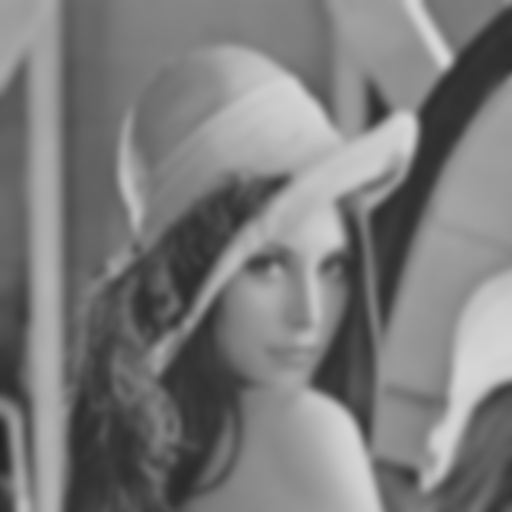
\includegraphics[width=2.5cm]{Lena_scales6.jpg}
				\caption{$\sigma = 2,15$, $N = 11$}
			\end{subfigure}
			\label{lena_scales}
		\end{center}
		\label{fig:as}
	\end{figure}
\end{frame}


%---------------------------------------------------------------------------
\begin{frame}
	\frametitle{Przetwarzanie obrazów w przestrzeni skali}

	Po wyznaczeniu reprezentacji skali dla obrazu można przeprowadzić dalsze operacje. W pracy zrealizowano detekcję:	
	\begin{figure}[h]
		\begin{center}
			\begin{subfigure}[b]{5cm}
				\centering
				\includegraphics[width=1cm]{blob.png}
				\caption{plam}
			\end{subfigure}
			~
			\begin{subfigure}[b]{5cm}
				\centering
				\includegraphics[width=1cm]{edge.png}
				\caption{krawędzi}
			\end{subfigure}

			\begin{subfigure}[b]{5cm}
				\centering
				\includegraphics[width=1cm]{corner.png}
				\caption{narożników}
			\end{subfigure}
			~
			\begin{subfigure}[b]{5cm}
				\centering
				\includegraphics[width=1cm]{ridge.png}
				\caption{grani}
			\end{subfigure}
		\end{center}
		\label{fig:asss}
	\end{figure}
\end{frame}

%---------------------------------------------------------------------------
\begin{frame}
	\frametitle{OpenCL}
	\begin{block}{OpenCL}
	\begin{tiny}
		Otwarty, wieloplatformowy standard pozwalający na wykorzystanie procesorów kart graficznych oraz innych urządzeń (w tym wielordzeniowe procesory CPU) w celu wykonywania obliczeń ogólnego przeznaczenia. Wykorzystanie karty graficznej pozwala na zrównoleglenie obliczeń.
	\end{tiny}
	\end{block}
	\begin{center}
	\includegraphics[width=3.5cm]{opencl.jpg}
	\end{center}
\end{frame}


%---------------------------------------------------------------------------
\begin{frame}[fragile]
	\frametitle{Użycie OpenCL do zrównoleglenia obliczeń}
	\begin{tiny}
	Do implementacji algorytmu z~wykorzystaniem OpenCL konieczne jest:
	\begin{itemize}
		\item Napisanie kodu kerneli - fragmentów kodu wykonywanych na karcie graficznej.
		\item Napisanie kodu wykonywanego na procesorze, który będzie kontrolował część wykonywaną na karcie graficznej. W tym zawiera się przekazanie parametrów do kerneli oraz pobranie wyników.
	\end{itemize}
	\end{tiny}

	\lstset{language=C,label=lis:edgeDetector,breaklines=true,basicstyle=\tiny\ttfamily}
	\begin{lstlisting}
__kernel void findLocalMax(__read_only image2d_t input, __write_only image2d_t output)
{
  int i = get_global_id(0);
  int j = get_global_id(1);

  float sum = read_imagef(input, sampler, (int2)(i, j)).x;
  for (int ii = -1; ii < 2; ++ii)
   for (int jj = -1; jj < 2; ++jj)
    if (read_imagef(input, sampler, (int2)(i + ii, j + jj)).x > sum)
      write_imageui(output, (int2)(i, j), 255);
    else
      write_imageui(output, (int2)(i, j), 0);
}
\end{lstlisting}



\end{frame}


%---------------------------------------------------------------------------
\begin{frame}
	\frametitle{Detekcja narożników}



	$$ k = |L_x^2L_{yy}  + L_y^2L_{xx} - 2L_xL_yL_{xy}| $$

	$ k $ - współczynnik krzywizny,

	$ L $ - pochodna wyznaczona z obrazu.

	%Po wyznaczeniu reprezentacji skali obrazu wykonywane są określone operacje matematyczne w~celu detekcji określonych struktur.

	Wzór przedstawia sposób detekcji narożników. Wyszukiwane są maksima lokalne wartości $ k $.


\end{frame}
%---------------------------------------------------------------------------
\begin{frame}
	\frametitle{Przykład detekcji plam}
%\includegraphics[trim=260 200 300 400, clip=true,width=\textwidth]{Operation/input.png}
	\begin{figure}[h]
		\begin{center}

			\begin{subfigure}[b]{5cm}
				\centering
				\includegraphics[trim=260 200 300 400, clip=true,width=\textwidth]{../Operation/input.png}
			\end{subfigure}~
			\begin{subfigure}[b]{5cm}
				\centering
				\includegraphics[trim=260 200 300 400, clip=true,width=\textwidth]{../Operation/blobResult.png}
			\end{subfigure}
		\end{center}
	\end{figure}
	
Obraz w skali 7.
	
\end{frame}
%---------------------------------------------------------------------------
\begin{frame}
	\frametitle{Przykład detekcji krawędzi}
%\includegraphics[trim=260 200 300 400, clip=true,width=\textwidth]{Operation/input.png}
	\begin{figure}[h]
		\begin{center}

			\begin{subfigure}[b]{5cm}
				\centering
				\includegraphics[trim=260 200 300 400, clip=true,width=\textwidth]{../Operation/input.png}
			\end{subfigure}~
			\begin{subfigure}[b]{5cm}
				\centering
				\includegraphics[trim=260 200 300 400, clip=true,width=\textwidth]{../Operation/edgeResult.png}
			\end{subfigure}
			
					\end{center}
	\end{figure}
	
	Obraz w skali 7.
\end{frame}
%---------------------------------------------------------------------------

\begin{frame}
	\frametitle{Przykład detekcji narożników}
%\includegraphics[trim=260 200 300 400, clip=true,width=\textwidth]{Operation/input.png}
	\begin{figure}[h]
		\begin{center}

			\begin{subfigure}[b]{5cm}
				\centering
				\includegraphics[trim=260 200 300 400, clip=true,width=\textwidth]{../Operation/input.png}
			\end{subfigure}~
			\begin{subfigure}[b]{5cm}
				\centering
				\includegraphics[trim=260 200 300 400, clip=true,width=\textwidth]{../Operation/cornerResult.png}
			\end{subfigure}
			\end{center}
	\end{figure}
	
	Obraz w skali 7.
\end{frame}
%---------------------------------------------------------------------------
\begin{frame}
	\frametitle{Przykład detekcji grani}
%\includegraphics[trim=260 200 300 400, clip=true,width=\textwidth]{Operation/input.png}
	\begin{figure}[h]
		\begin{center}

			\begin{subfigure}[b]{5cm}
				\centering
				\includegraphics[trim=260 200 300 400, clip=true,width=\textwidth]{../Operation/input.png}
			\end{subfigure}~
			\begin{subfigure}[b]{5cm}
				\centering
				\includegraphics[trim=260 200 300 400, clip=true,width=\textwidth]{../Operation/ridgeResult.png}
			\end{subfigure}
			\label{fig:wynik}
		\end{center}
	\end{figure}
	
	Obraz w skali 7.

\end{frame}
%---------------------------------------------------------------------------
\begin{frame}
	\frametitle{Poprawność rozwiązania}

	Na podstawie porównania z implementacją realizowaną na procesorze CPU stwierdzono, że wykonanie algorytmu na karcie graficznej daje poprawne wyniki.

	Największe rozbieżności są na poziomie 2\%, w~większości przypadków nie przekraczają 1\%.
	\begin{tiny}
	\begin{table}[h]
\begin{tabular}{|l|l|l|l|l|l|}
\hline
Nr skali & Reprezentacja skali & Detekcja plam & Detekcja krawędzi & Detekcja narożników & Detekcja grani \\ \hline
1        & 0.05                & 0.70          & 0.06              & 0.03                & 0.10           \\ \hline
2        & 0.08                & 0.84          & 0.03              & 0.01                & 0.35           \\ \hline
3        & 0.11                & 0.68          & 0.02              & 0.01                & 0.63           \\ \hline
4        & 0.14                & 0.55          & 0.01              & 0.00                & 0.75           \\ \hline
5        & 0.17                & 0.48          & 0.01              & 0.00                & 0.89           \\ \hline
6        & 0.20                & 0.61          & 0.00              & 0.00                & 1.12           \\ \hline
7        & 0.23                & 0.41          & 0.00              & 0.00                & 1.29           \\ \hline
8        & 0.26                & 0.32          & 0.00              & 0.00                & 1.56           \\ \hline
9        & 0.28                & 0.45          & 0.00              & 0.00                & 1.75           \\ \hline
10       & 0.31                & 0.34          & 0.00              & 0.00                & 1.83           \\ \hline
\end{tabular}
\end{table}
\end{tiny}

\end{frame}
%---------------------------------------------------------------------------
\begin{frame}
	\frametitle{Szybkość rozwiązania}

	\begin{center}
		\includegraphics[width=10cm]{../TestySzybkosci/PureAGH.png}
	\end{center}
\tiny{Z pomiarów czasu obliczeń można zauważyć, że obliczenia na karcie graficznej Nvidia GeForce GTX 670 trwały krócej.}

\end{frame}
%---------------------------------------------------------------------------

\begin{frame}
	\frametitle{}
	\begin{center}
		Dziękuję za uwagę.
	\end{center}
\end{frame}
